\documentclass[12pt]{article}
%[10pt,technote]{IEEEtran}
\usepackage{hyperref}
\usepackage{graphicx}
\usepackage[affil-it]{authblk}
\usepackage{color}
\usepackage{amsgen,amsmath,amstext,amsbsy,amsopn,amssymb}
\usepackage{geometry}
\usepackage{subcaption}
\usepackage{caption}
\usepackage{wrapfig}
\usepackage{comment}
\usepackage{mathrsfs}
\usepackage{upgreek}
\usepackage{amssymb}
\usepackage{textcomp}
\usepackage{amsmath}
\usepackage{tcolorbox}
\usepackage{listings}
\usepackage{fancyhdr}
\usepackage{cite}
\usepackage{wasysym} 
%\usepackage{subfigure}
%\usepackage{wraptable}

\geometry{left=2.5cm, right=2.5cm,top=2.5cm,bottom=2.5cm}



\setcounter{secnumdepth}{0}
\title{\bf Homework 4}
\author{Jiani Gao\\jgao30@binghamton.edu}
\affil{Department of Economics, Binghamton University}
\date{\today}
\pagestyle{fancy}
\chead{Econ634 hw4} \lhead{}\rhead{}
\cfoot{jgao30@binghamton.edu}

\begin{document}
\maketitle
\newpage
\tableofcontents	

\newpage

\section{Step 1: Frim's problem}

Firm's problem now is:
\[\max\limits_{\{K_{t+1}^d,N_t^d\}}\sum\limits_{t=0}^\infty(\frac{1}{\prod_{i=0}^{t} r_i})\pi (K,N;w_t,r_t)=\max\limits_{\{K_{t+1}^d,N_t^d\}}\sum\limits_{t=0}^\infty(\frac{1}{\prod_{i=0}^{t} r_i})(K_t^\alpha N_t^{1-\alpha}-w_t N_t-r_t K_{t}+(1-\delta)K_t) \tag{1}
\]	
By doing the first order condition with respect to $K_{t+1}$ and $N_t$, we can get the following conditions:

\[\alpha K_{t+1}^{\alpha -1}N_{t+1}^{1-\alpha}=r_{t+1}+\delta-1
\tag{2}
\]
\[(1-\alpha)K_t^\alpha N_t^{-\alpha}=w_t\tag{3}
\]
Equation (2) also holds for period t, so we should also have that 
\[\alpha K_{t}^{\alpha -1}N_{t}^{1-\alpha}=r_{t}+\delta-1
\tag{4}
\]
\section{Step 2: Household value function}
The household choose $c_t$ and $a_{t+1}$ to maximize the expected utlity, or we can write $c_t$ as a function of $a_{t+1}$ so that we can write down the value function as:
\[v(z_t,a_t)=\max\limits_{a_{t+1}}U(c_t)+\beta  E v(z_{t+1},a_{t+1})\tag{5}
\]
where $c_t=z_tw_t\bar{l}+r_ta_t-a_{t+1}$, and the utility function is CRRA utility function.

\section{Step 3: Discretize the exogenous state variable}
For $\rho=0.5$, $\sigma_\epsilon=0.2$ and number of z equals to 5, we can get a discrete set of possible values for z:
\[z=\begin{bmatrix}
0.5002&0.7072&1.0000&1.4140&1.9993
\end{bmatrix}\tag{6}
\]
we can also get the invatiant distribution from $m\times m$ transition matrix:
\[\pi^{inv}(z)=\begin{bmatrix}
0.0145&0.2189&0.5333& 0.2189& 0.0145

\end{bmatrix}\tag{7}
\]
So the aggregate labor supply $N^s=1.0338$
\section{Step 4: Discretize the endogenous state variable}
In this step, we discretize a into a grid with 500 points. At this time, I choose $a_{max}=5$, and we will adjust this number later according to the binding constraint.
\section{Step 5: Solving the model numerically}
From Step 3, we know that $N^s=1.0338$, thus $N_d=1.0338$ due to market clear condition. Now let's guess $K=2$, and using equation (3) and equation (4), we can calculate the value for $r$ and $w$.\\\\
\[r_{t}=\alpha K_{t}^{\alpha -1}N_{t}^{1-\alpha}+1-\delta \tag{8}\]
\[w_t=(1-\alpha)K_t^\alpha N_t^{-\alpha} \tag{9}\]
\noindent
Please see the Appendix for Matlab code.

\section{Step 6: Analyze the results}
\begin{enumerate}


	\item [a.] The steady state interest rate I get is $r=1.0928$, while in the complete market case $r^{CM}=1/\beta=1.0101$. So interest rate in the incomplete market is higher. Why???
    \item [b.] Below is the policy functions for m productivity series:
    \begin{figure}[!h]\centering
	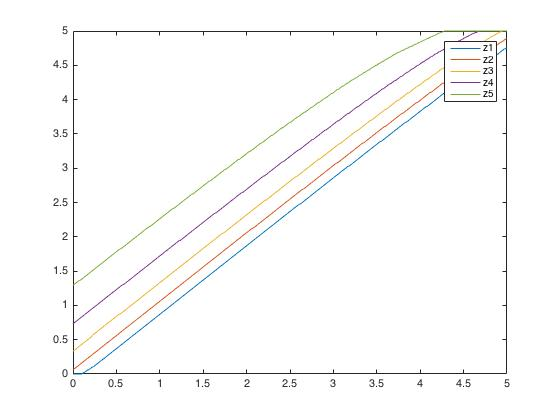
\includegraphics[width=6in,height=5in]{policy}
    \end{figure}
    \item [c.]This time we take asset holding as wealth(why?), and the Lorenz curve is:
    \begin{figure}[!h]\centering
    	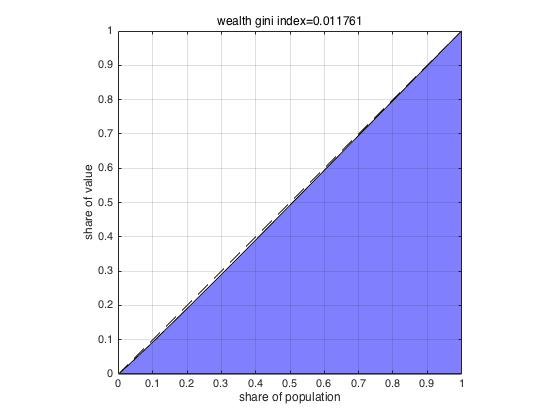
\includegraphics[width=5in,height=5in]{wgini}
    \end{figure}
    \newline The gini index is smaller comparing with gini index in Hugget model.
\end{enumerate}
\section{Step 7: Alternative way of coding}
Solving the value function on a coarse grid, and using the result as a starting value. Then use policy function iteration.\\\\
For this approach, runtime is  .While the runtime is  when using valur funtion iteration.\\\\
Please see appendix.

\section{Appendix: Matlab code}
    \subsection{Way 1}
     \begin{verbatim}
     %%%%%%%%%parameters%%%%%%%%
     alpha=1/3;
     beta=0.99;
     s=2;
     delta=0.025;
     
     
     %%%%%question 3%%%%%%%%%%%%%%%%%%%%%%%%%%%%%
     m=5;
     rho=0.5;
     sigma=0.2;
     d=3;
     
     [z,zprob] =TAUCHEN(m,rho,sigma,d);
     z=exp(z);
     pi=zprob^1000;
     pz=pi(1,:);
     ns=pz*z;
     %%%%%%%question 4%%%%%%%%%%%%%%%%%%%%%%%%%%%%
     a_min=0;
     a_max=5;
     a_num=500;
     a=linspace(a_min,a_max,a_num);
     %%%%%%question 5%%%%%%%%%%%%%%%%%%%%%%%%%%%%%
     nd=ns;
     k_guess=2;
     
     d=1;
     while d>=0.001;
     r=alpha*k_guess^(alpha-1)*nd^(1-alpha)+1-delta;
     w=(1-alpha)*k_guess^alpha*nd^(-alpha);
     
     %consumption fn
     cons=bsxfun(@minus,r*a',a);
     cons=bsxfun(@plus,cons,permute(w*z,[2 3 1]));
     %return fn
     ret=cons.^(1-s)/(1-s);
     ret(cons<0)=-Inf;
     %value fn and policy fn
     v_guess=zeros(m,a_num);
     v_tol = 1;
     while v_tol >.0001;
     % CONSTRUCT RETURN + EXPECTED CONTINUATION VALUE
     
     vf=bsxfun(@plus,ret,permute(beta*zprob*v_guess,[3,2,1]));
     
     % CHOOSE HIGHEST VALUE (ASSOCIATED WITH a' CHOICE)
     [vfn,pol_indx]=max(vf,[],2);
     v_tol=[max(abs(vfn(:,:,1)' - v_guess(1,:))) ; max(abs(vfn(:,:,2)' - v_guess(2,:)));...
     max(abs(vfn(:,:,3)' - v_guess(3,:)));max(abs(vfn(:,:,4)' - v_guess(4,:)));...
     max(abs(vfn(:,:,5)' - v_guess(5,:)))];
     v_guess=[vfn(:,:,1)';vfn(:,:,2)';vfn(:,:,3)';vfn(:,:,4)';vfn(:,:,5)'];
     end;
     % KEEP DECSISION RULE
     pol_indx=permute(pol_indx, [3 1 2]);
     pol_fn=a(pol_indx); 
     % SET UP INITITAL DISTRIBUTION
     Mu=ones(m,a_num)/(m*a_num);
     
     % ITERATE OVER DISTRIBUTIONS
     m_tol=1;
     while m_tol>0.0001
     [z_ind, a_ind, mass] = find(Mu > 0); % find non-zero indices
     
     MuNew = zeros(size(Mu));
     
     
     for ii = 1:length(z_ind)
     apr_ind = pol_indx(z_ind(ii), a_ind(ii)); % which a prime does the policy fn prescribe?
     MuNew(:, apr_ind) = MuNew(:, apr_ind) +[zprob(z_ind(ii),1)*Mu(z_ind(ii),a_ind(ii));zprob(z_ind(ii),2)*Mu(z_ind(ii),a_ind(ii));zprob(z_ind(ii),3)*Mu(z_ind(ii),a_ind(ii));zprob(z_ind(ii),4)*Mu(z_ind(ii),a_ind(ii));zprob(z_ind(ii),5)*Mu(z_ind(ii),a_ind(ii))];
     % which mass of households goes to which exogenous state?
     end
     m_tol=max(max(abs(MuNew-Mu)));
     Mu=MuNew;
     end     
     
     aggsav=Mu(1,:)*a'+Mu(2,:)*a'+Mu(3,:)*a'+Mu(4,:)*a'+Mu(5,:)*a';
     d=abs(k_guess-aggsav);
     if k_guess<aggsav
     k_guess=k_guess+abs(k_guess-aggsav)/2;
     else k_guess=k_guess-abs(k_guess-aggsav)/2;
     end
     k_guess;
     d;
     end
     
     %%%%%%%%%question 6
     plot(a,pol_fn(1,:),a,pol_fn(2,:),a,pol_fn(3,:),a,pol_fn(4,:),a,pol_fn(5,:)),legend('z1','z2','z3','z4','z5');
     
     %gini
     p=[Mu(1,:);Mu(2,:);Mu(3,:);Mu(4,:);Mu(5,:)];
     wealth=[a;a;a;a;a];
     wg=gini(p,wealth,true);
     title(['wealth gini index=',num2str(wg)]);
     
     
     \end{verbatim}


%\bibliographystyle{unsrt} 
%\bibliography{}
\end{document}
